\documentclass{article}



\usepackage{graphicx}                       % Pacchetti

\usepackage[italian]{babel}

\graphicspath{ {./images/} }

\usepackage{imakeidx}

\usepackage{hyperref}%



\makeindex[columns=1, title=Tavola dei contenuti, intoc]



\begin{document}

	\begin{titlepage}

		\begin{center}

			\huge\textbf{Montani Website}\\

			\Large\textbf{5 INB}\\

			\Large \textbf{Manuale d'uso}\\

			\vspace{4cm}

			\large Project Manager: \textbf{Boussoufa Yacine}\\

			\large Data: \textbf{05/03/2022}\\

			\large Versione: \textbf{0.1}\\

		\end{center}

	\end{titlepage}

	\clearpage

	\begin{tabular}{ |p{1cm}|p{4cm}|p{3cm}|p{2cm}|  }

		\hline

		\multicolumn{4}{|c|}{Cronologia delle revisioni} \\

		\hline

		ID& Cambiamenti &Data di creazione&Autore\\

		\hline

		1&Creazione&05/03/2022&Boussoufa Yacine\\

		\hline

	\end{tabular}

	

	\clearpage


	\tableofcontents
	

	\index{generate}

	\clearpage
	

	%Stampa del titolo, autore e data


	\textbf{{\fontsize{5mm}{10mm}\selectfont \section{Introduzione} }}

	\begin{flushleft}
		L'Istituto Tecnico Tecnologico Statale “G. e M. MONTANI” di Fermo ha commissionato una modernizzazione grafica e funzionale del sito web dell'Istituto, il quale non rispetta i requisiti grafici e funzionali, definiti dal modello standard di siti web scolastici realizzato dal Team per la Trasformazione Digitale, su richiesta del Ministero dell’Istruzione.\\
		In riferimento alla Direttiva 8/09 del Ministro per la Pubblica Amministrazione e l'Innovazione, è necessario rispettare quanto specificato all'articolo 4 della direttiva in termini di "Linee Guida per i siti Web della PA" e il "Vademecum". \\
		Il fine di queste linee guida è quello di raggiungere gli obiettivi di gestione, sviluppo e diffusione previsti dalla normativa.\\
	\end{flushleft}

	\vspace{3mm}

	\subsection{\textbf{Interfaccia}}

		Il sito web è stato realizzato attraverso il software di gestione di contenuti (CMS) Wordpress basato su PHP,che permette una gestione facilitata attraverso una dashboard.
		Wordpress operando su un web server, e un database, consente la creazione di un sito, formato da contenuti testuali e multimediali, gestibili ed aggiornabili in maniera dinamica: facendo uso di codice HTML, CSS e Javascript.\\
		Wordpress permette anche l'installazione di plugin e temi in modo da personalizzare ulteriormente il sito.\\

	\vspace{3mm}

	\pagebreak

	\textbf{{\fontsize{5mm}{10mm}\selectfont \section{Wordpress} }}

	\subsection{\textbf{Dashboard}}
	La dashboard di WordPress è la prima schermata che verrà visualizzata dopo aver effettuato l'accesso come amministratore del sito, e permetterà la visualizzazione della panoramica del sito web raccogliendo un vasto numero di gadgets che forniscono le principali informazioni dell'intero sito. La Dashboard può essere personalizzata in base alle esigenze dell'utente e in base ai plugin installati.
	
	\vspace{0.5 cm}

	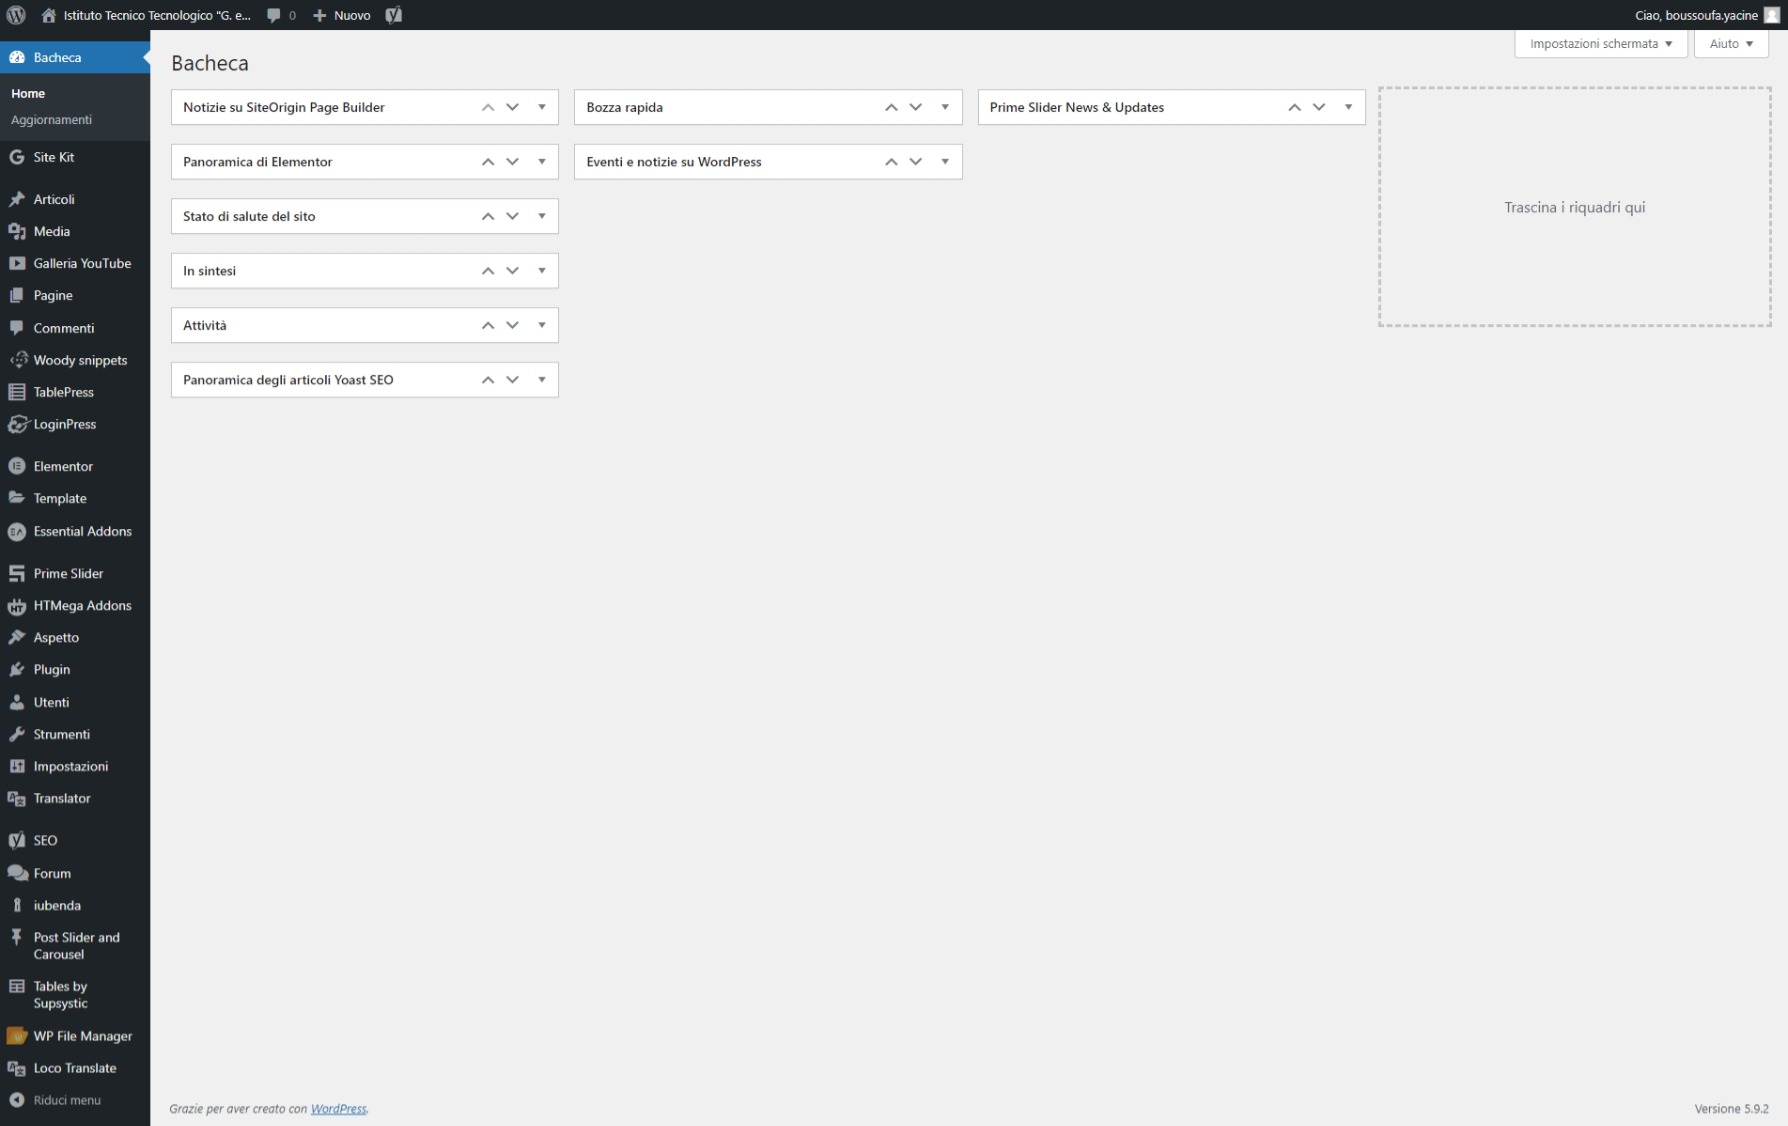
\includegraphics[scale=0.18]{Dashboard Wordpress.jpeg}

	\subsection{\textbf{Tema}}

	\subsection{\textbf{Plugin}}

	\subsection{\textbf{Impostazioni aggiuntive}}

	\pagebreak
	
	\textbf{{\fontsize{5mm}{10mm}\selectfont \section{Pagine} }}

	\subsection{\textbf{Creazione nuova pagina}}

	\subsection{\textbf{Elementor}}

	Le pagine dell'intero sito sono realizzate utilizzando un Page Builder denominato 'Elementor': questo ha il vantaggio di poter essere utilizzato senza dover intervenire manualmente su tutto il codice della singola pagina.
	Questa tipologia di editor permette di vedere le modifiche al sito man mano che vengono eseguite rendendo più facile e immediata la creazione dell'intero sito.
	Procedento alla creazione di una nuova pagina, sarà quindi necessario fare click sul pulsante 'Modifica con Elementor'.

	\vspace{0.5 cm}

	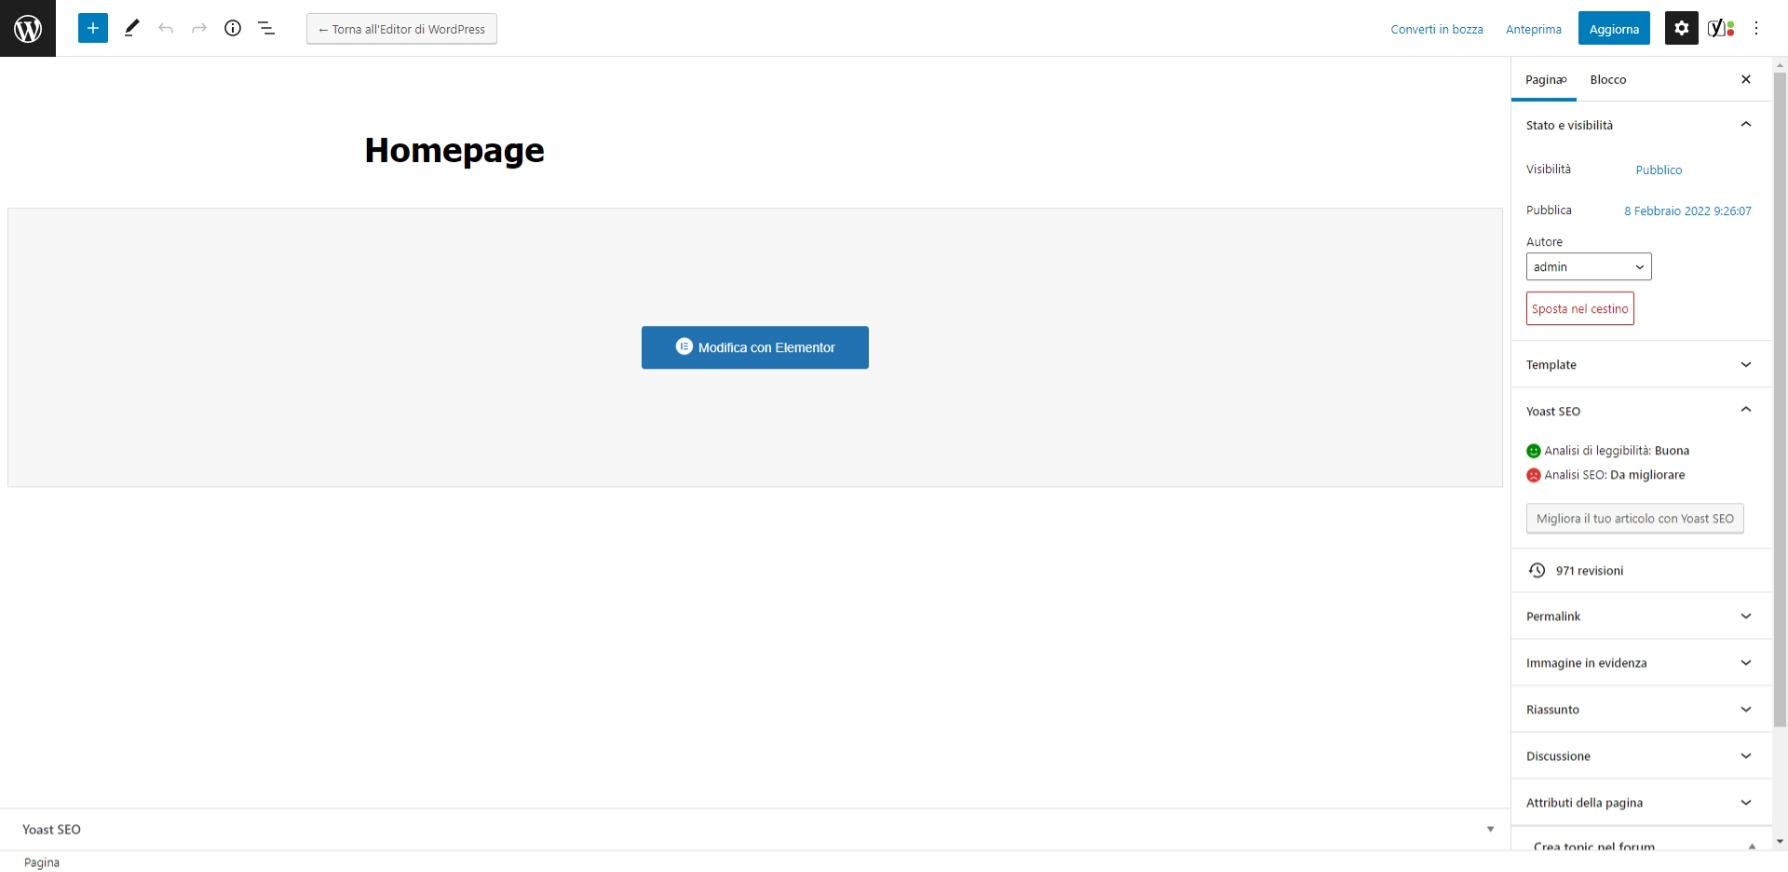
\includegraphics[scale=0.18]{Modifica con Elementor.jpeg}

	\vspace{0.5 cm}

	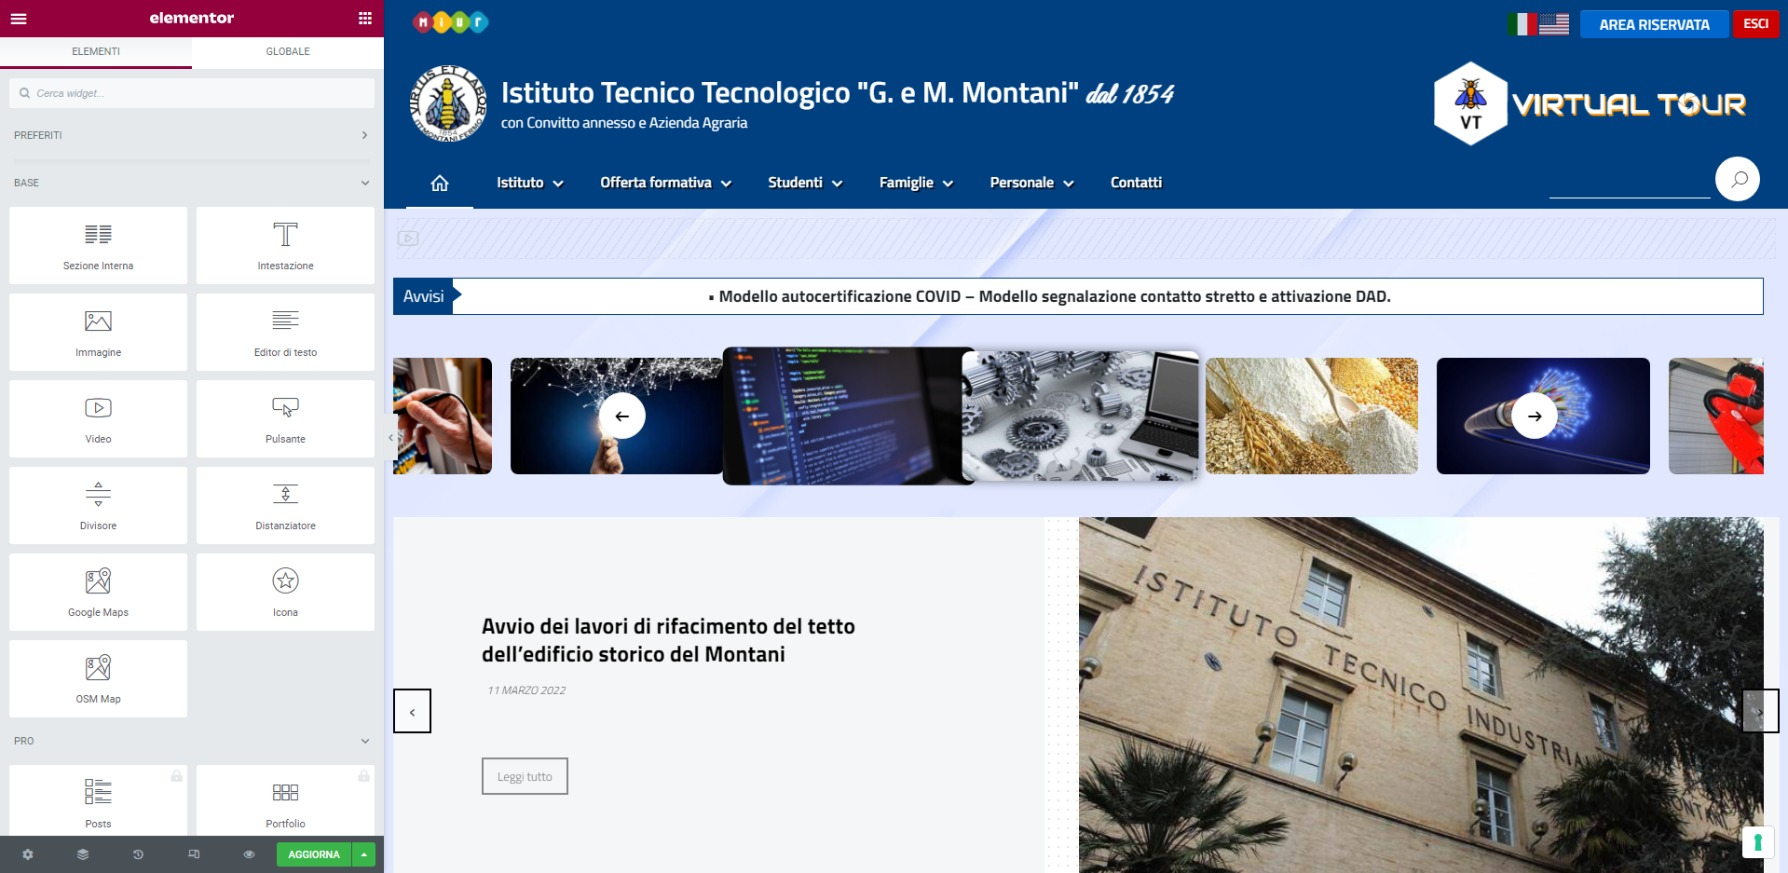
\includegraphics[scale=0.18]{Elementor.jpeg}

	\subsection{\textbf{Homepage}}
	Come sopra indicato, anche il contenuto della Homepage è stata realizzata utilizzando Elementor ed è strutturato come segue:
	\begin{itemize}
		\item Slider Avvisi;
		\item Slider Indirizzi;
		\item Slider Notizie in evidenza;
		\item Colonna News
		\item Colonna "Servizi"
		\item PON
	\end{itemize}	

		\subsubsection{\textbf{Slider Avvisi}}
			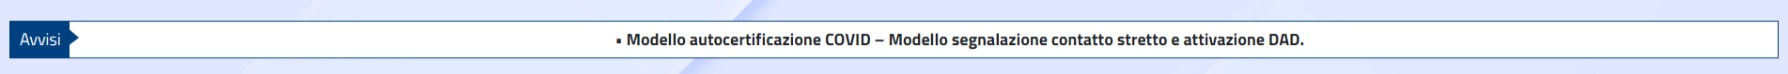
\includegraphics[scale=0.19]{Slider Avvisi.jpeg}\\
			Lo slider degli Avvisi è modificabile attraverso il blocco di Elementor ed è stato generato da codice HTML e da un CSS personalizzato:
			Questo codice è modificabile nelle prime righe del blocco ed è rappresentato da un'unica lista identificata dal tag 'ul' e da una serie di elementi identificati dal tag 'li'. All'interno di quest'ultimo è presente un collegamento attraverso il tag 'a href' che permeete di inserire un testo visualizzabile e un collegamento ipertestuale.\\
			
			\vspace{0.2 cm}
			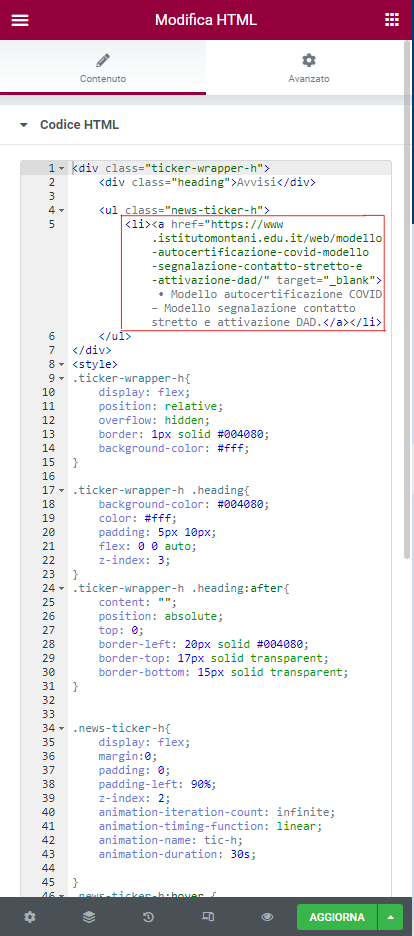
\includegraphics[scale=0.28]{Modifica Slider Avvisi.png}\\
		\subsubsection{\textbf{Slider Indirizzi}}
		\subsubsection{\textbf{Slider Notizie in evidenza}}
		\subsubsection{\textbf{Colonna News}}
		\subsubsection{\textbf{Colonna "Servizi"}}
		\subsubsection{\textbf{PON}}


	\subsection{\textbf{Forum}}

	\subsection{\textbf{Indirizzi}}

	\subsection{\textbf{Webinar}}

	\subsection{\textbf{Repository}}
		\subsubsection{\textbf{Libri di Testo}}
		\subsubsection{\textbf{Modulistica}}
		\subsubsection{\textbf{Programmazioni}}

	

	\pagebreak

	\textbf{{\fontsize{5mm}{10mm}\selectfont \section{Articoli} }}

	\subsection{\textbf{Categorie}}


\end{document}